\documentclass[ucs]{beamer}
\usepackage{polski}
\usepackage[utf8]{inputenc}
\usepackage{pgfplots}
\usepackage{tikz}
\usetikzlibrary{automata,positioning,shapes,shadows,arrows,backgrounds,trees,fit,calc,decorations.pathreplacing,decorations.markings}

\usetheme{Ilmenau}
%\usetheme{Marburg}

\title{Gas Analyzer \newline aplikacja do analizatorów wykorzystująca protokół ELAN}
\subtitle[Współpraca międzywydziałowa]{Projekt zrealizowany w ramach współpracy między \newline Wydziałem Automatyki, Elektroniki i Informatyki, a \newline Wydziałem Inżynierii Środowiska i Energetyki}

\author[Karbowiak, Powała]{mgr inż. Damian Karbowiak  \and mgr inż. Grzegorz Powała}
\institute[Politechnika Śląska]{\includegraphics[height=0.2\textheight]{images/PolslLogo} }
\date{\today}
       
\setbeamertemplate{footline}[frame number]
\useoutertheme{infolines}
 
\begin{document}

\begin{frame}
  \titlepage
\end{frame}


\section{Wstęp}
\begin{frame}
\frametitle{Historia}
\begin{itemize}
\setlength{\itemsep}{5pt}
\setlength{\parskip}{5pt}
\setlength{\parsep}{5pt}
\item 22 luty 2013 \\
Kontakt mailowy ze strony mgr inż. Tomasz Kress
\item 28 luty 2013 \\
Pierwsze spotkanie w celu omówienia problemu i zadania
\item 21 marzec 2013 \\
Wypożyczenie Ultramatu 23 i rozpoczęcie współpracy oraz realizacji projektu
\item kwiecień -- czerwiec 2013 \\
Realizacja projektu
\item wrzesień 2013 \\
Finalizacja pierwszej części i podstawowej wersji projektu
\end{itemize}
\end{frame}

\begin{frame}
\frametitle{Współpraca}
\begin{center}
\begin{tabular}{cccccc}
\includegraphics[width=0.1\textwidth]{images/AEiILogo} &
\includegraphics[width=0.1\textwidth]{images/IILogo} &
\includegraphics[width=0.25\textwidth]{images/SKNIndustrumLogo} &
\includegraphics[width=0.1\textwidth]{images/WISiELogo} &
\includegraphics[width=0.1\textwidth]{images/IMIUELogo} &
\includegraphics[width=0.1\textwidth]{images/ZKiWPLogo} \\ 
\end{tabular} 
\end{center}

\begin{enumerate}
\setlength{\itemsep}{3pt}
\setlength{\parskip}{3pt}
\setlength{\parsep}{3pt}
\item Wydział Automatyki, Elektroniki i Informatyki
\begin{itemize}
\setlength{\itemsep}{3pt}
\setlength{\parskip}{3pt}
\setlength{\parsep}{3pt}
\item Instytut Informatyki
\begin{itemize}
\setlength{\itemsep}{3pt}
\setlength{\parskip}{3pt}
\setlength{\parsep}{3pt}
\item Koło Naukowe Przemysłowych Zastosowań Informatyki ,,Industrum''
\\ mgr inż. Damian Karbowiak
\\ mgr inż. Grzegorz Powała
\end{itemize}
\end{itemize}
\item  Wydział Inżynierii Środowiska i Energetyki
\begin{itemize}
\setlength{\itemsep}{3pt}
\setlength{\parskip}{3pt}
\setlength{\parsep}{3pt}
\item Instytut Maszyn i Urządzeń Energetycznych
\begin{itemize}
\setlength{\itemsep}{3pt}
\setlength{\parskip}{3pt}
\setlength{\parsep}{3pt}
\item Zakład Kotłów i Wytwornic Pary
\\ mgr inż. Tomasz Kress
\end{itemize}
\end{itemize}
\end{enumerate}
\end{frame}


\section{Współpraca}
\begin{frame}
\frametitle{Możliwości}
\begin{enumerate}
\setlength{\itemsep}{3pt}
\setlength{\parskip}{3pt}
\setlength{\parsep}{3pt}
\item Instytut Informatyki
\begin{itemize}
\setlength{\itemsep}{2pt}
\setlength{\parskip}{2pt}
\setlength{\parsep}{2pt}
\item Wiedza informatyczna
\item Specjalizacja związana ze stosowaniem informatyki w przemyśle
\item Koło naukowe o tematyce przemysłowej
\item Projekty zaliczeniowe semestralne oraz prace inżynierskie i magisterskie
\item Studenci chętni do realizacji projektów praktycznych z wykorzystaniem istniejącego sprzętu i stanowisk laboratoryjnych
\end{itemize} 
\item Instytut Maszyn i Urządzeń Energetycznych
\begin{itemize}
\setlength{\itemsep}{2pt}
\setlength{\parskip}{2pt}
\setlength{\parsep}{2pt}
\item Potrzeba informatyzacji
\item Ciekawe problemy informatyczne
\item Spora ilość sprzętu i stanowisk
\item Ciekawe pomysły i potrzeby na oprogramowanie/sprzęt
\end{itemize}
\end{enumerate}
\end{frame}

\begin{frame}
\frametitle{Gas Analyzer - geneza}
\begin{enumerate}
\setlength{\itemsep}{5pt}
\setlength{\parskip}{5pt}
\setlength{\parsep}{5pt}
\item Realizacja pomiarów przemysłowych
\item Wykorzystywanie kilku analizatorów firmy SIEMENS
\item Zapisywanie pomiarów w tabelce na kartce
\item Ograniczona częstotliwość pomiarów
\end{enumerate}
\end{frame}

\begin{frame}
\frametitle{Przykładowy wynik pomiarów}
\begin{center}
\includegraphics[width=0.99\textheight]{images/IMG_4559}
\end{center}
\end{frame}

\begin{frame}
\frametitle{Przykładowa kartka z pomiarem}
\begin{center}
\includegraphics[width=0.99\textheight]{images/IMG_4562}
\end{center}
\end{frame}

\begin{frame}
\frametitle{Gas Analyzer - realizacja}
\begin{enumerate}
\item Wykorzystanie protokołu komunikacyjnego ELAN
\item Możliwość podłączenia do 12 analizatorów firmy SIEMENS:
\begin{itemize}
\item ULTRAMAT 6
\item OXYMAT 6 / OXYMAT 61
\item CALOMAT 6
\item ULTRAMAT 23
\end{itemize}
\item Automatyczny odczyt stanu urządzeń
\item Możliwość archiwizacji pomiarów z dowolnym interwałem czasowym, z~rozdzielczością co sekundę
\item Automatyczne wykrywanie urządzeń i wielkości mierzonych
\item Konfigurowalna precyzja pomiarów (wyświetlanie i raporty)
\item Generowanie raportów do PDF oraz XLS
\item Niskie koszty uruchomienia
\end{enumerate}
\end{frame}

\begin{frame}
\frametitle{ELAN -- Podłączenie}
\begin{figure}[htbp]
 \centering
        \tikzstyle{background grid}=[draw, black!50,step=.25cm]
	\begin{tikzpicture}[scale=0.2]%, show background grid]
	\tikzset{
    	mynode/.style={rectangle,rounded corners,draw=black, top color=white, bottom color=yellow!50,very thick, inner sep=1em, minimum size=3em, 		text centered, text width=3.3cm},
    	mynodemini/.style={rectangle,rounded corners,draw=black, top color=white, bottom color=yellow!50,very thick, inner sep=.5em, text centered},    	
	    myarrow/.style={->, >=latex', shorten >=1pt, thick},
	    myline/.style={-, =latex', shorten >=1pt, rounded corners, ultra thick},
	    mylabel/.style={text width=7em, text centered} 
	} 
	\node[mynode] (plc) {Komputer \\ przemysłowy C6925};  
	\node [left=of plc] (laptop) {\includegraphics[width=3cm]{images/laptop}};
	\node[below=2cm of plc] (dummy) {}; 
	\node[mynode, left=of dummy] (io) {Wyspa EK1100 z~zestawem modułów IO};  	 	 	
 	\node[mynodemini, left=of io] (io2) {EL1004};
 	\node[mynodemini, above=2mm of io2] (io1) {EL4132};  	
 	\node[mynodemini, above=2mm of io1] (io0) {EK1100};
 	\node[mynodemini, below=2mm of io2] (io3) {EL2004}; 	 	
 	\node[mynodemini, below=2mm of io3] (io4) {EL2004};
 	\node[mynodemini, below=2mm of io4] (io5) {EL3102};
 	\node [fit=(io0) (io1) (io2) (io3) (io4) (io5)] (fit) {};  
 	%\draw [decorate, xshift=-20pt,line width=4pt] (fit.south east) -- (fit.north east);
	\draw [decorate,decoration={brace, mirror,amplitude=10pt}, line width=1pt] (fit.south east) -- (fit.north east);
	
	\node[mynode, right=of dummy] (naped) {Napęd\\serwomechnizmów AX5203};
	\node[below=2cm of naped] (dummy2) {}; 
	\node[mynode, left=of dummy2, text width=4cm](silnik1){Silnik \\ AM3021-0C00-0000};
	\node[mynode, right=of dummy2, text width=4cm](silnik2){Silnik \\ AM3021-0C40-0000};
	
	\draw[myline,black,dotted] (fit.east) ++(0.4, 0) -- (io.west);
	\draw[myline,blue] (laptop.east) -- ++(-1, 0) -- (plc.west);
	
	\draw[myline,purple] (io0.south) -- (io1.north);	
	\draw[myline,purple] (io1.south) -- (io2.north);
	\draw[myline,purple] (io2.south) -- (io3.north);		
	\draw[myline,purple] (io3.south) -- (io4.north);
	\draw[myline,purple] (io4.south) -- (io5.north);
	
	\draw[myline,yellow] (plc.south) -- (naped.north);	
	\draw[myline,yellow] (io.east) -- (naped.west);	

	\draw[myline, green, bend right=10] (naped.south) to (silnik1.north);
	\draw[myline, orange, bend left=10] (naped.south) to (silnik1.north);	
	\draw[myline, green, bend right=10] (naped.south) to (silnik2.north);
	\draw[myline, orange, bend left=10] (naped.south) to (silnik2.north);	
	%\draw[<->, >=latex', shorten >=2pt, shorten <=2pt, bend right=45, thick, dashed] 
    %(io.south) to node[auto, swap] {Competition}(naped.south); 
    
	\draw [fill=blue!5, thick] (5.75,1.5) rectangle (9,-3);

    \draw [purple, line width=6] (6,1) -- (6.5,1); \node[text width=2cm] at (7.65,0.7) {EtherCAT (E-bus)};    
    \draw [yellow, line width=6] (6,0) -- (6.5,0); \node[text width=2cm] at (7.65,-0.3) {EtherCAT (skrętka)};
    \draw [blue, line width=6] (6,-1) -- (6.5,-1); \node at (7.5,-1) {Ethernet};
    \draw [black, line width=6] (6,-1.5) -- (6.5,-1.5); \node at (7.5,-1.5) {Zasilanie};
    \draw [green, line width=6] (6,-2) -- (6.25,-2); \draw [orange, line width=6] (6.25,-2) -- (6.5,-2); 
    \node [text width=2cm] at (7.75,-2.25) {Sterowanie silnikiem};    
\end{tikzpicture} 
\caption{Schemat stanowiska typu CP.}
\label{stanowisko:cp}
\end{figure}
\end{frame}

\begin{frame}
\frametitle{ELAN Network zasada działania buforów}
\tikzstyle{background grid}=[draw, black!50,step=.25cm]
\newcounter{wavenum}
\newcounter{iter}

\setlength{\unitlength}{1cm}

% advance clock one cycle, not to be called directly
\newcommand*{\clki}[1]{
  \draw[white] (t_cur) -- ++(#1,0) node[time] (t_cur) {};
}

\newcommand*{\bitvector}[3]{
  \draw[fill=#3] (t_cur) -- ++( .1, .3) -- ++(#2-.2,0) -- ++(.1, -.3)
                         -- ++(-.1,-.3) -- ++(.2-#2,0) -- cycle;
  \path (t_cur) -- node[anchor=mid] {#1} ++(#2,0) node[time] (t_cur) {};
}

% \known{val}{length}
\newcommand*{\known}[2][]{
    \bitvector{#1}{#2}{white}
}

% \unknown{length}
\newcommand*{\unknown}[2][]{
    \bitvector{#1}{#2}{black!30}
}

% \bit{1 or 0}{length}
\newcommand*{\bit}[2]{
  \draw (t_cur) -- ++(0,.6*#1-.3) -- ++(#2,0) -- ++(0,.3-.6*#1)
    node[time] (t_cur) {};
}
\newcommand*{\lbl}[2]{
 \path (t_cur) -- node[time] {} ++(#2-.2,0) node[anchor=mid] (t_cur) {#1} ++(.2,0) node[time] (t_cur) {};
}

% \nextwave{name}
\newcommand{\nextwave}[1]{
  \path (0,\value{wavenum}) node[left=0.5cm] {#1} node[time] (t_cur) {};
  \addtocounter{wavenum}{-1}
}

\newcommand{\nr}{
	$\Rightarrow$
}

\newcommand{\ur}{
	$\circlearrowleft$
}

% \clk{name}{period}
\newcommand{\clk}[2]{
    \nextwave{#1}
    \FPeval{\res}{(\wavewidth+1)/#2}
    \FPeval{\reshalf}{#2/2}
    \foreach \t in {1,2,...,\res}{
        \bit{\reshalf}{1}
        \bit{\reshalf}{0}
    }
}
    
% \begin{wave}[clkname]{num_waves}{clock_cycles}
\newenvironment{wave}[3][]{
  \begin{tikzpicture}[draw=black, yscale=.7,xscale=1]%, show background grid]
    \tikzstyle{time}=[coordinate]
    \setlength{\unitlength}{1cm}
    \def\wavewidth{#3}
    \setcounter{wavenum}{0}
    \nextwave{#1}
    \def\myarray{1,5,1}
    %\foreach \t in {0,1,...,\wavewidth}{
    \foreach \i / \x in {0/1.5, 1/2, 2/1.25, 3/2.5, 4/.75, 5/1, 6/1.75} {
      \draw[dotted] (t_cur) +(0,.1) node[above] {$t_\i$} -- ++(0,.4-#2);
      \clki{\x};
    }
    \draw[->, >=latex', shorten >=1pt, thick] (-.4,-3.5) -- (-.4,0);
    \draw[->, >=latex', shorten >=1pt, thick] (-.4,-3.5) -- (10,-3.5);
}
{\end{tikzpicture}}

\begin{wave}{4}{15}
 \nextwave{Bufor 1}  \lbl{\nr}{0} \known{.5} \lbl{}{1} \unknown{.5} \lbl{\ur}{1.5} \unknown{.5} \lbl{}{.75} \unknown{.5} \lbl{}{2} \unknown{.5} \lbl{}{1.25} \known{.5}
 \nextwave{Bufor 2}  \known{.5} \lbl{}{1} \known{.5} \lbl{}{1.5} \known{.5} \lbl{\nr}{.75} \known{.5} \lbl{}{2} \unknown{.5} \lbl{\nr}{1.25} \known{.5}
 \nextwave{Bufor 12} \known{.5} \lbl{\nr}{1} \known{.5}	\lbl{}{1.5} \unknown{.5} \lbl{}{.75} \unknown{.5} \lbl{\ur}{2} \unknown{.5} \lbl{}{1.25} \known{.5}
\end{wave}

$t_0$ -- nadejście pomiaru z urządzenia 1 \\
$t_1$ -- nadejście pomiaru z urządzenia 12 \\
$t_2$ -- nadejście pomiaru z urządzenia 1 \\
$t_3$ -- nadejście pomiaru z urządzenia 2 \\
$t_4$ -- nadejście pomiaru z urządzenia 12 \\
$t_5$ -- MIGAWKA \\
$t_6$ -- nadejście pomiaru z urządzenia 2 
\end{frame}

\begin{frame}
\frametitle{ELAN Network zasada działania buforów}
\begin{figure}[htbp]
 \centering
        \tikzstyle{background grid}=[draw, black!50,step=.25cm]
	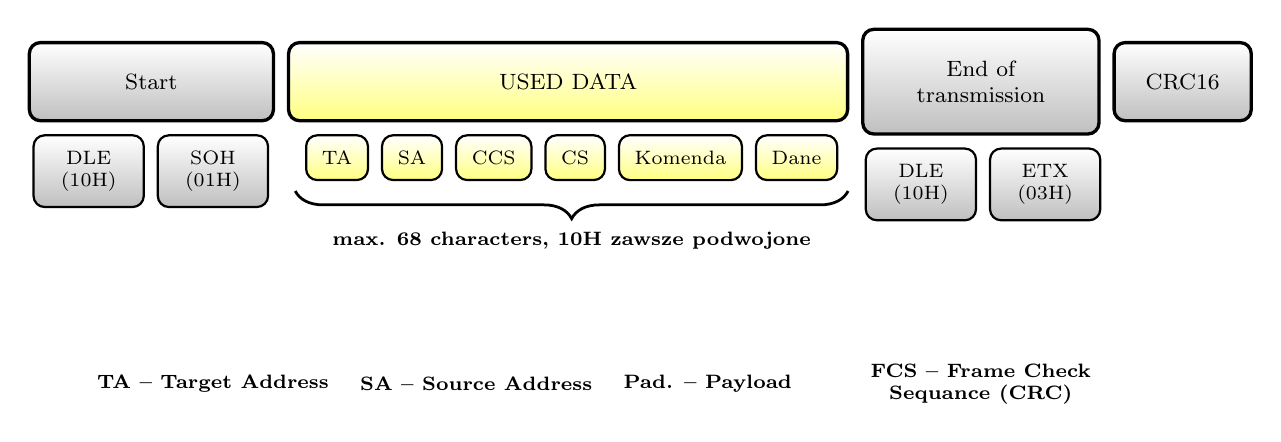
\begin{tikzpicture}[node distance=1.5mm, auto]%, show background grid]
	\tikzset{
    	mynode/.style={rectangle,rounded corners,draw=black, top color=white, very thick, inner sep=4mm, 		text centered,font=\footnotesize},
    	mynodemini/.style={rectangle,rounded corners,draw=black, top color=white, thick, inner sep=2mm, text centered,font=\scriptsize},    	
	    myarrow/.style={->, >=latex', shorten >=1pt, ultra thick},
	    myline/.style={-, =latex', shorten >=1pt, rounded corners, ultra thick},
	    mylabel/.style={text centered, font=\scriptsize\bfseries} 
	} 
	\node[bottom color=gray!50, mynode, text width=2.3cm] (start) {Start};  
	\node[bottom color=gray!50, mynodemini, below=of start.213, text width=1cm] (dle) {DLE (10H)};	
	\node[bottom color=gray!50, mynodemini, right=of dle, text width=1cm] (soh) {SOH (01H)};  
	
	\node[bottom color=yellow!50, mynode, right=of start, text width=6.3cm] (used_data) {USED DATA};
	\node[bottom color=yellow!50, mynodemini, below=of used_data.190] (ud1) {TA};  	 
	\node[bottom color=yellow!50, mynodemini, right=of ud1] (ud2) {SA};
	\node[bottom color=yellow!50, mynodemini, right=of ud2] (ud3) {CCS};
	\node[bottom color=yellow!50, mynodemini, right=of ud3] (ud4) {CS};
	\node[bottom color=yellow!50, mynodemini, right=of ud4] (ud5) {Komenda};
	\node[bottom color=yellow!50, mynodemini, right=of ud5] (ud6) {Dane};			

	\node [fit=(ud1) (ud2) (ud3) (ud4) (ud5) (ud6)] (fit) {};  
 	%\draw [decorate, xshift=-20pt,line width=4pt] (fit.south east) -- (fit.north east);
	\draw [decorate,decoration={brace,amplitude=10pt}, line width=1pt] (fit.south east) -- (fit.south west);		
	\node[mylabel, below=4mm of fit] (fits) {max. 68 characters, 10H zawsze podwojone};
			
	\node[bottom color=gray!50, mynode, right=of used_data, text width=2.2cm] (eot) {End of \\ transmission};
	\node[bottom color=gray!50, mynodemini, below=of eot.222, text width=1cm] (dle2) {DLE (10H)};
	\node[bottom color=gray!50, mynodemini, right=of dle2, text width=1cm] (etx) {ETX (03H)}; 	 
	
	\node[bottom color=gray!50, mynode, right=of eot] (crc16) {CRC16};
	
	\node[mylabel, below=2cm of soh] (dal) {TA -- Target Address};
	\node[mylabel, right=of dal] (sal) {SA -- Source Address};
	\node[mylabel, right=of sal] (padl) {Pad. -- Payload};
	\node[mylabel, right=of padl, text width=4cm] (fcsl) {FCS -- Frame Check Sequance (CRC)};			
	
\end{tikzpicture} 
\caption{Ramka w protokole ELAN.}
\label{elan:ramka}
\end{figure}
\end{frame}

\begin{frame}
\frametitle{ELAN Network zasada działania buforów}
\resizebox{260pt}{!}{
	\begin{tikzpicture}[node distance=2mm,auto]
	\tikzset{
    	mynode/.style={rectangle,rounded corners,draw=black, top color=white, very thick, inner sep=3mm, 		text centered,font=\footnotesize},
	    myarrow/.style={ <->, shorten >=1pt, line width=1mm},
	    myarrow1/.style={ ->, line width=0.4mm},	    
   	    myarrow2/.style={ ->, shorten >=1mm, line width=0.4mm},
   	    myarrow3/.style={ ->, shorten >=4mm, line width=0.4mm},   	    
	    mylabel/.style={text centered, font=\scriptsize\bfseries} 
	} 
	\node[bottom color=blue!60, mynode, text width=12cm] (gui) {Graficzny interfejs użytkownika};  
	\node[bottom color=blue!60, mynode, text width=12cm, text height=2.5cm, below=.75cm of gui] (elanNetwork) {Moduł ELAN Network}; 
	\node[bottom color=gray!40, mynode, text width=2cm, below=3cm of gui.173] (a) {Detekcja ramek}; 
	\node[bottom color=gray!40, mynode, text width=2cm, right=of a] (b) {Weryfikacja ramek}; 
	\node[bottom color=gray!40, mynode, text width=2cm, right=of b] (c) {Parsowanie ramek}; 	
	\node[bottom color=gray!40, mynode, text width=2cm, right=of c] (d) {Budowanie migawki}; 
	\node[bottom color=blue!60, mynode, text width=12cm, below=.75cm of elanNetwork] (rxtx) {Biblioteka RXTX}; 
	\node[bottom color=blue!60, mynode, text width=12cm, below=.75cm of rxtx] (conv) {Konwerter RS485 $\Leftrightarrow$ USB};   		
	\node[bottom color=blue!60, mynode, text width=12cm, below=.75cm of conv] (devices) {Urządzenia pomiarowe};	

	\draw[myarrow] (gui.south) -- (elanNetwork.north) node [midway,black] {Przetworzone dane};
	\draw[myarrow] (elanNetwork.south) -- (rxtx.north) node [midway,black] {Odczyt bajtów};	
	\draw[myarrow] (rxtx.south) -- (conv.north) node [midway,black] {USB};	
	\draw[myarrow] (conv.south) -- (devices.north) node [midway,black] {RS485};
	\draw[myarrow1] (a) -- (b);
	\draw[myarrow1] (b) -- (c);
	\draw[myarrow1] (c) -- (d);	
	\draw[myarrow2] (c.north) -- (elanNetwork.north) node [midway,black] {};
	\draw[myarrow3] (d.north) -- (elanNetwork.north) node [midway,black] {};
\end{tikzpicture}
}
\end{frame}

\begin{frame}
\frametitle{ELAN Network zasada działania buforów}
\tikzstyle{abstract}=[rectangle, draw=black, rounded corners, fill=blue!40, drop shadow,
        text centered, anchor=north, text=white, text width=4cm]
\tikzstyle{comment}=[rectangle, draw=black, rounded corners, fill=green, drop shadow,
        text centered, anchor=north, text=white, text width=4cm]
\tikzstyle{myarrow}=[->, >=open triangle 90, thick]
\tikzstyle{line}=[-, thick]

\begin{figure}[!htb] 	
\centering 	
\begin{tikzpicture}[node distance=1.1cm]
    \node (GasAnalyzer) [abstract, rectangle split, rectangle split parts=2]
        {
            \textbf{GasAnalyzer}
            \nodepart{second}wersja 0.1.0
        };
	\node (AuxNode01) [text width=4cm, below=of GasAnalyzer] {};
    \node (ELANNetwork) [abstract, rectangle split, rectangle split parts=2, left=of AuxNode01]
        {
            \textbf{ELANNetwork}
            \nodepart{second}wersja 0.1.0
        };
    \node (GasAnalyzerGUI) [abstract, rectangle split, rectangle split parts=2, right=of AuxNode01]
        {
            \textbf{GasAnalyzerGUI}
            \nodepart{second}wersja 0.1.0
        };    
    \draw[myarrow] (ELANNetwork.north) -- ++(0,0.1) -| (GasAnalyzer.south);
    \draw[line] (ELANNetwork.north) -- ++(0,0.1) -| (GasAnalyzerGUI.north); 
        
\end{tikzpicture}
\caption{Struktura projektu} 
\label{projectSchema}
 \end{figure}
\end{frame}

\begin{frame}
\frametitle{Podgląd sieci}
\includegraphics[width=0.99\textwidth]{images/detailNetworkW}
\end{frame}

\begin{frame}
\frametitle{Podgląd urządzenia}
\includegraphics[width=0.99\textwidth]{images/detailDeviceW}
\end{frame}

\begin{frame}
\frametitle{Przykładowy raport PDF}
\includegraphics[width=0.9\textwidth]{images/pdf}
\end{frame}

\begin{frame}
\frametitle{Przykładowy raport XLS}
\includegraphics[width=0.99\textwidth]{images/xls}
\end{frame}

\section{Podsumowanie}
\begin{frame}
\frametitle{Wnioski}
\begin{itemize}
\setlength{\itemsep}{5pt}
\setlength{\parskip}{5pt}
\setlength{\parsep}{5pt}
\item Liczne perspektywy współpracy
\item Aktywizacja studentów
\item Rozwiązywanie praktycznych problemów i zadań
\item Utworzenie stałego kanału współpracy 
\item Pozytywne postrzeganie dążenia do współpracy i wymiany doświadczeń
\end{itemize}
\end{frame}

\begin{frame}
\frametitle{Podsumowanie oraz pytania}
Dziękujemy za uwagę.
\\\vspace{2cm}
Czas na pytania.
\\\vspace{2cm}
mgr inż. Damian Karbowiak -- Damian.Karbowiak@polsl.pl\\
mgr inż. Grzegorz Powała -- Grzegorz.Powala@polsl.pl
\end{frame}

\end{document}